\section{Problema}
\subsection{Contexto y delimitación de la necesidad}
La información de interés estudiantil se distribuye mediante grupos de mensajería, redes sociales, portales, correo y murales. La coexistencia de canales no constituye por sí misma una falla; la dificultad aparece cuando el usuario no identifica el aviso válido, lo encuentra tarde o debe consultar varios lugares para completar una misma gestión.

\subsection{Formulación del problema central}
El problema es el \textbf{acceso disperso y poco oportuno a información académica y administrativa relevante para la comunidad de la escuela}. La encuesta describe dependencia de medios informales, fechas importantes no conocidas a tiempo y valoración desfavorable del acceso a la información. Las fotografías muestran soportes físicos de difusión y las plantas permiten estudiar ubicaciones; no cuantifican por sí solas demoras o pérdidas de oportunidades.

\subsection{Causas, efectos y evidencia}
\cuadro{tab:problema}{Problema, causas y efectos por contrastar}{@{}P{3.0cm}Y Y@{}}{\textbf{Dimensión}&\textbf{Condición o causa propuesta}&\textbf{Efecto y verificación}}{
Origen de avisos & Publicaciones distribuidas entre canales con distinta autoridad & Dificultad para reconocer la versión válida; revisar avisos y fuentes\\*
Gestión editorial & Responsables, aprobación y caducidad por precisar & Riesgo de avisos atrasados o vencidos; verificar flujo de publicación\\
Acceso & Canales poco visibles o difíciles de localizar & Búsqueda adicional y fechas omitidas declaradas; observar consultas\\
Continuidad & Dependencia de red, alimentación y soporte & Riesgo de indisponibilidad; registrar incidencias y probar recuperación\\
Colaboración & Oportunidades y proyectos con visibilidad limitada & Interés en conectar equipos; comprobar uso efectivo\\
}
La línea base verificará tiempos de búsqueda, vigencia de avisos, responsables y disponibilidad. Estas variables permitirán contrastar las causas y medir el cambio del servicio.

\subsection{Árbol de problemas}
La figura \ref{fig:arbol_problemas} ordena las condiciones del cuadro \ref{tab:problema}. Las causas directas sostienen el problema central y éste produce efectos observables que convergen en un efecto final. Cada relación es una hipótesis de trabajo; la línea base verificará su magnitud.

\begin{center}
\begin{tikzpicture}[x=1cm,y=1cm,>=Latex,
  caja/.style={draw,rounded corners=3pt,align=center,inner sep=4pt,line width=0.6pt,font=\footnotesize,text width=2.52cm,minimum height=2.0cm,execute at begin node={\setstretch{1.0}\hyphenpenalty=10000\exhyphenpenalty=10000}},
  efecto/.style={caja,fill=unsaacrojo!7,draw=unsaacrojo!55},
  causa/.style={caja,fill=black!5,draw=black!40},
  central/.style={draw=unsaacrojo,fill=unsaacrojo,text=white,rounded corners=3pt,align=center,inner sep=5pt,font=\small\bfseries,text width=14.6cm,minimum height=1.5cm,execute at begin node={\setstretch{1.0}\hyphenpenalty=10000\exhyphenpenalty=10000}},
  final/.style={draw=unsaacrojo!70,fill=unsaacrojo!20,rounded corners=3pt,align=center,inner sep=4pt,line width=0.6pt,font=\footnotesize\bfseries,text width=14.6cm,minimum height=1.25cm,execute at begin node={\setstretch{1.0}\hyphenpenalty=10000\exhyphenpenalty=10000}},
  rotulo/.style={rotate=90,font=\scriptsize\bfseries,text=graytext,align=center},
  flecha/.style={->,draw=black!50,line width=0.7pt}]
\node[final] (fin) at (8.32,7.95) {Menor aprovechamiento de oportunidades académicas y profesionales, trámites y colaboración en la comunidad de la EPIIS};
\node[efecto] (e1) at (2.2,5.7) {Dificultad para reconocer el aviso válido};
\node[efecto] (e2) at (5.26,5.7) {Avisos atrasados o vencidos en circulación};
\node[efecto] (e3) at (8.32,5.7) {Búsqueda en varios canales y fechas omitidas\\[1pt]{\scriptsize\color{graytext}81,7\% las declara}};
\node[efecto] (e4) at (11.38,5.7) {Interrupciones de consulta sin recuperación};
\node[efecto] (e5) at (14.44,5.7) {Baja visibilidad de proyectos y oportunidades};
\node[central] (pc) at (8.32,3.35) {Acceso disperso y poco oportuno a información académica y administrativa relevante para la comunidad de la EPIIS};
\node[causa] (c1) at (2.2,1.0) {Canales con distinta autoridad\\[1pt]{\scriptsize\color{graytext}79,3\% WhatsApp o Facebook}};
\node[causa] (c2) at (5.26,1.0) {Sin responsables, aprobación ni caducidad definidos};
\node[causa] (c3) at (8.32,1.0) {Consulta poco visible en espacios comunes};
\node[causa] (c4) at (11.38,1.0) {Acceso dependiente de red, energía y soporte};
\node[causa] (c5) at (14.44,1.0) {Proyectos y oportunidades sin canal de difusión};
\foreach \n in {1,...,5}{
  \draw[flecha] (c\n.north) -- (c\n.north |- pc.south);
  \draw[flecha] (e\n.south |- pc.north) -- (e\n.south);
  \draw[flecha] (e\n.north) -- (e\n.north |- fin.south);
}
\node[rotulo] at (0.35,7.95) {EFECTO\\FINAL};
\node[rotulo] at (0.35,5.7) {EFECTOS};
\node[rotulo] at (0.35,3.35) {PROBLEMA};
\node[rotulo] at (0.35,1.0) {CAUSAS};
\end{tikzpicture}
\captionof{figure}{Árbol de problemas del servicio de información de la EPIIS}\label{fig:arbol_problemas}
\end{center}

\subsection{Entorno de difusión}
Los soportes físicos de información forman parte del entorno que atenderá el servicio. El piloto integrará avisos de estos canales con publicaciones digitales y una gestión común de vigencia.
% Las tres fotografías comparten una fila para que la figura no se divida entre páginas.
\par\vspace{4pt}\noindent\begin{minipage}{\linewidth}\centering
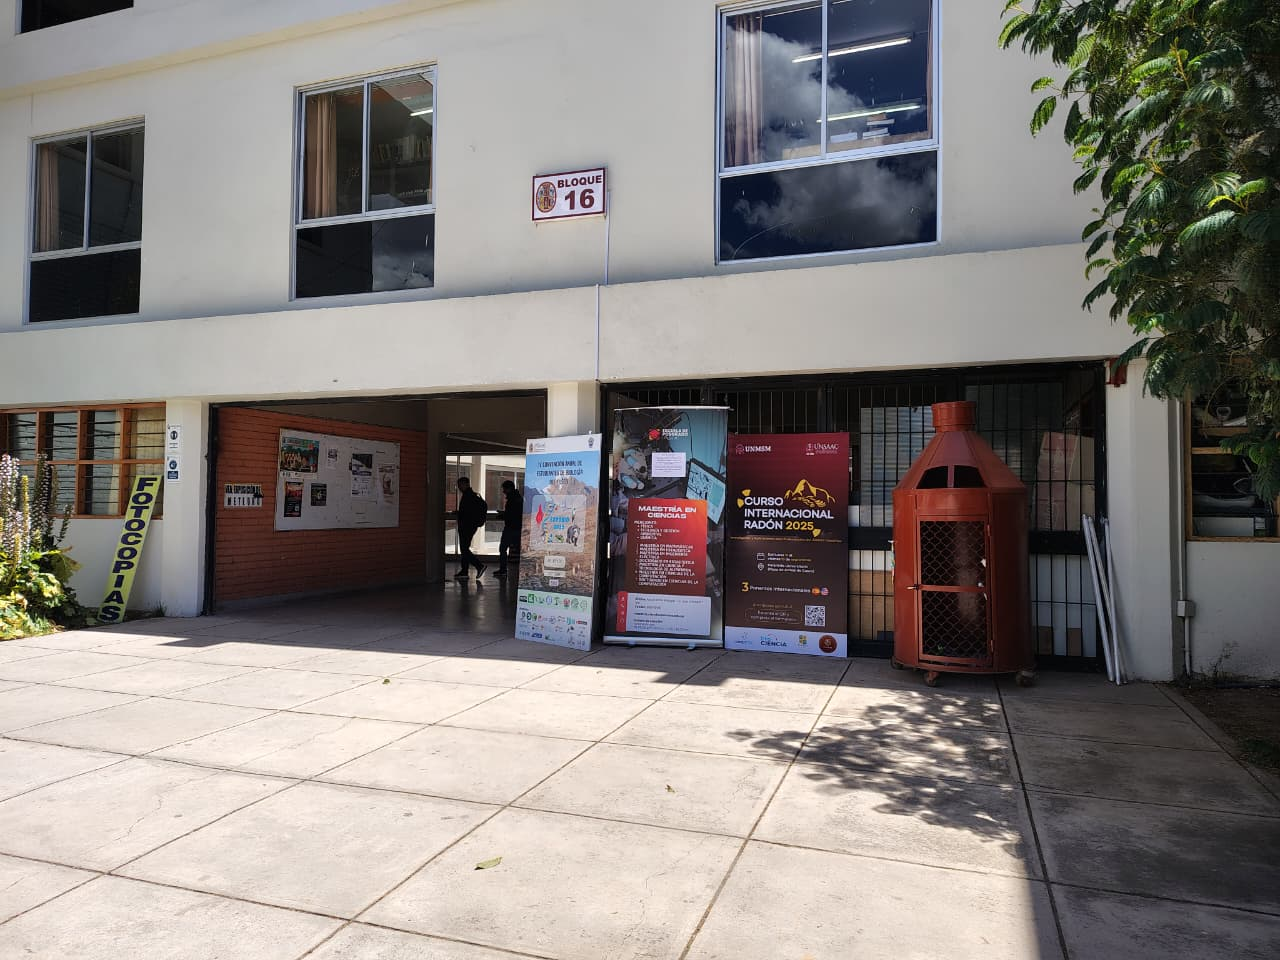
\includegraphics[height=4.4cm,keepaspectratio]{imagenes/foto_ingreso.png}\hfill
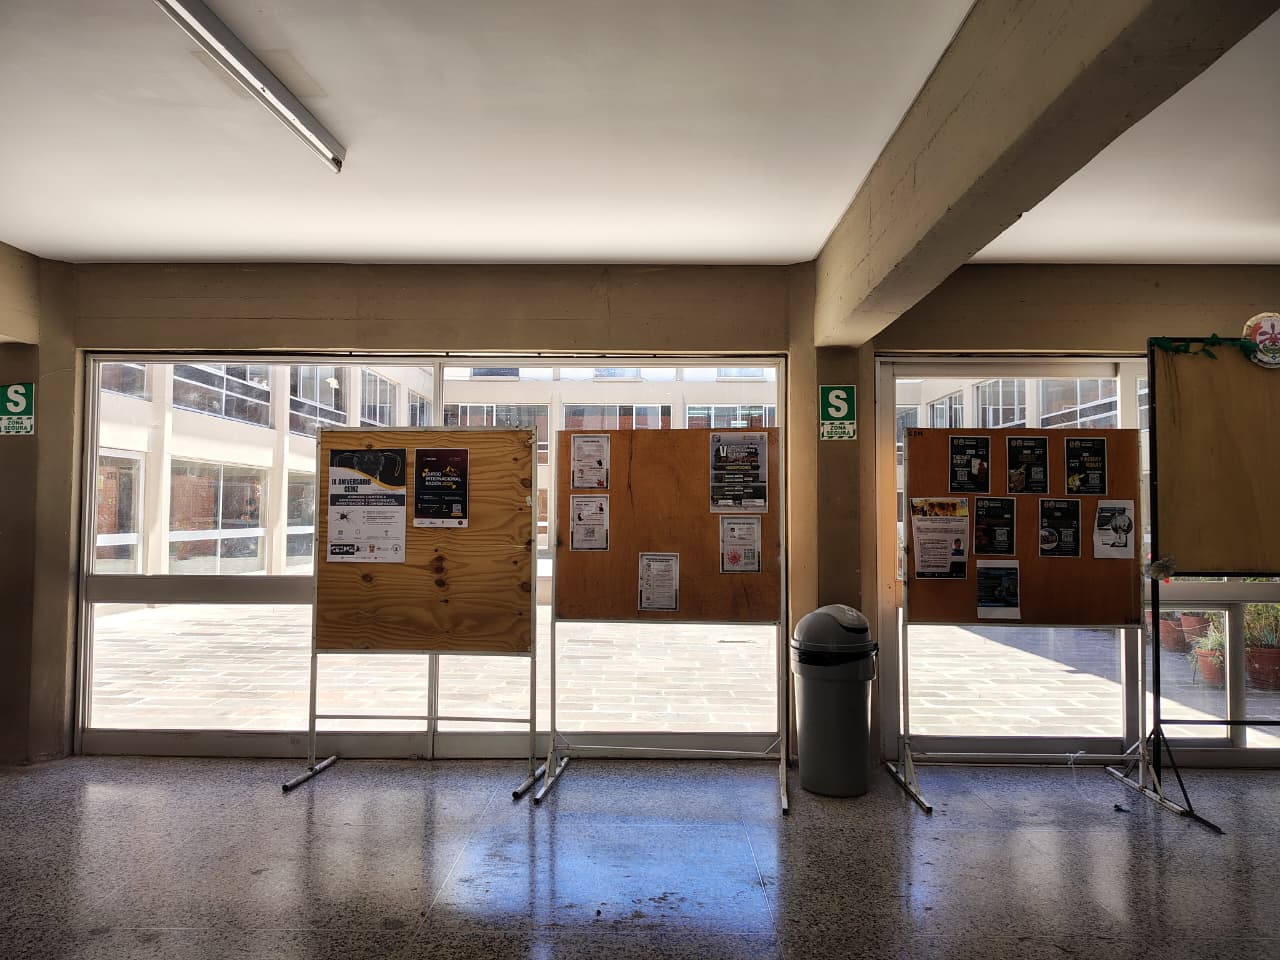
\includegraphics[height=4.4cm,keepaspectratio]{imagenes/foto_murales.png}\hfill
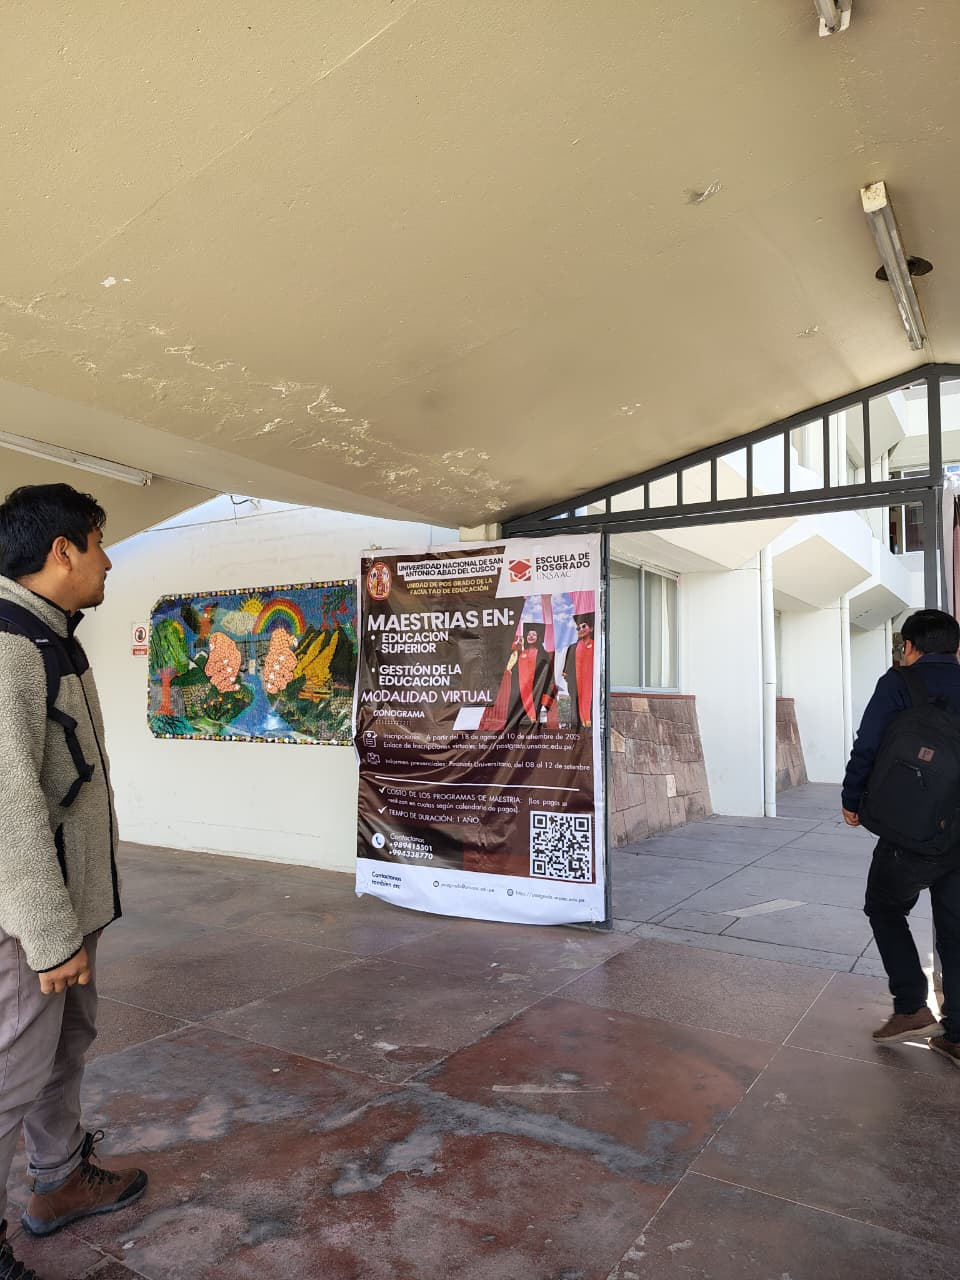
\includegraphics[height=4.4cm,keepaspectratio]{imagenes/foto_pasillo.png}\par
\captionof{figure}{Entorno de difusión: ingreso, murales y pasillos}\label{fig:entorno}
\end{minipage}\par\vspace{4pt}

\section{Origen del proyecto}
La iniciativa se origina en la necesidad de articular la información que llega a la comunidad estudiantil por distintos medios y convertirla en un servicio de consulta confiable. Las respuestas sobre fechas omitidas, acceso a avisos y formatos preferidos orientan esa necesidad; no demuestran que una tecnología particular sea la única respuesta.

El componente informático surge de la oportunidad de gestionar el ciclo completo del aviso: emisor, validación, publicación, vigencia, destino y seguimiento. La consulta táctil y el QR se plantean como alternativas complementarias para acceder a esa información desde espacios comunes y dispositivos personales.

El componente solar se evalúa por aporte energético, continuidad y costo de ciclo de vida. Su incorporación exige comparar el servicio con respaldo de red y la variante con generación FV, bajo iguales funciones y objetivos de disponibilidad.

Los porcentajes del cuadro \ref{tab:origen} corresponden a la base gráfica de \textbf{300 respuestas de varias escuelas}, de las cuales 76 pertenecen a Ingeniería Informática y de Sistemas. No se dispone de cruces individuales para calcular esos resultados sólo para la EPIIS; por tanto, describen al conjunto de respuestas y orientan la validación local.

\cuadro{tab:origen}{Origen y fundamento de las decisiones de diseño}{@{}P{3.1cm}Y Y@{}}{\textbf{Necesidad o condición}&\textbf{Evidencia disponible}&\textbf{Decisión propuesta}}{
Acceso oportuno & 81,7\% declara haber omitido alguna fecha por falta de información & Centralizar avisos y validar el tiempo de consulta\\*
Fuente reconocible & 79,3\% usa principalmente WhatsApp o Facebook & Mostrar emisor, fuente oficial, revisión y vigencia\\
Consulta accesible & Preferencias táctil 60,7\% y QR 31,7\% & Probar terminales y continuidad en móvil; conservar otros canales\\
Gestión de contenidos & Riesgo de duplicidad y desactualización por contrastar & Establecer responsables y flujo editorial antes de automatizar\\
Aporte y respaldo energético & Cargas y condiciones del sitio pendientes & Comparar red/respaldo con FV híbrida dimensionada\\
}

\section{Finalidad pública}

El proyecto busca facilitar a la comunidad de la EPIIS el acceso a información institucional oportuna, verificable y comprensible. Se concentra en oportunidades académicas y profesionales, fechas de trámites, eventos y proyectos de colaboración. Un servicio bien gestionado puede reducir búsquedas innecesarias y ampliar la visibilidad de oportunidades, sin sustituir los canales oficiales ni limitar el acceso de quienes no se encuentren en el pabellón.

La intervención integra proceso editorial, software, terminales públicos, conectividad y alimentación eléctrica. La utilidad pública reside en que el usuario encuentre información válida y pueda actuar sobre ella. La pantalla y el sistema solar son medios para prestar ese servicio, cuya conveniencia se evaluará con resultados medibles y recursos sostenibles.

El ámbito inicial comprende tres ubicaciones interiores de la EPIIS, una por piso. La expansión se organizará por edificios después de evaluar resultados del piloto, infraestructura y capacidad de contenido y soporte.

\subsection{Sustento normativo y exigencias de calidad}
La finalidad no descansa sólo en la preferencia de los usuarios. El cuadro \ref{tab:normativa} relaciona las obligaciones legales y los estándares de acreditación con lo que el servicio debe cumplir. Los artículos citados de la Ley Universitaria se verificaron en su texto publicado \cite{ley30220}; los estándares corresponden al modelo de acreditación de programas universitarios del SINEACE aprobado en 2025 \cite{sineace2025}.

\cuadro{tab:normativa}{Sustento normativo y de acreditación del servicio}{@{}P{3.3cm}Y Y@{}}{\textbf{Norma o estándar}&\textbf{Disposición pertinente}&\textbf{Exigencia para el proyecto}}{
Ley N.° 30220, art. 11 & Publicar en forma permanente y actualizada, entre otros, becas y créditos disponibles (11.4) y número de alumnos por programa (11.8) & Difundir avisos oficiales con fuente y vigencia, y enlazar al portal de transparencia\\*
Ley N.° 30220, art. 100 & Ambientes y equipos accesibles para personas con discapacidad (100.8); uso de los servicios académicos y de bienestar (100.10) & Altura, aproximación, contraste y alternativa QR; consulta libre y gratuita\\
Ley N.° 30220, art. 126 & Programas de bienestar para la comunidad universitaria & Difundir becas, salud, eventos y servicios de apoyo\\
SINEACE 2025, estándares 5 y 8 & Recursos e infraestructura tecnológica; gestión de la información para decidir y mejorar & Registros de uso, vigencia y desempeño exportables como evidencia\\
SINEACE 2025, estándares 6 y 7 & Responsabilidad social y desarrollo sostenible; bienestar y servicios de apoyo & Medición del aporte FV y difusión de servicios estudiantiles\\
Ley N.° 32069 y su Reglamento, num. 44.6 & El requerimiento no menciona marca, fabricante ni procedencia, salvo compatibilización aprobada & Especificaciones genéricas ET-01 a ET-10; marcas sólo en la indagación\\
Ley N.° 29733 y D.S. N.° 016-2024-JUS & Tratamiento de datos personales y videovigilancia & Consulta sin datos personales; cámaras con aviso, finalidad y conservación limitadas\\
CNE, Utilización & Seguridad de instalaciones eléctricas interiores & Protecciones, tierra y caída de tensión verificadas por profesional\\
Régimen RAEE & Gestión de residuos de aparatos eléctricos y electrónicos & Retiro trazable de equipos y baterías\\
}
Las normas y estándares se citan en \cite{contrataciones,compatibilizacion,datos,cne,raee}. La universidad no tiene equipamiento previo de este tipo que justifique una compatibilización. Por ello el requerimiento se redacta por desempeño y cualquier marca que cumpla la especificación puede ofertar.

\subsection{Estadísticas e insumos de la formulación}
Cada cifra que usa el informe proviene de una fuente identificada. El cuadro \ref{tab:insumos} reúne los insumos que determinan alcance, demanda, energía y costo, e indica cómo se reemplazarán cuando exista el dato institucional.

\cuadro{tab:insumos}{Estadísticas e insumos utilizados y su fuente}{@{}P{3.4cm}P{3.0cm}Y@{}}{\textbf{Insumo}&\textbf{Valor}&\textbf{Fuente y actualización}}{
Estudiantes de la EPIIS & 830 a 870 & Matrícula referencial del equipo; confirmar con registro oficial 2026-II\\*
Respuestas de la encuesta & 300; 76 de la EPIIS & Base gráfica del instrumento, anexo A\\
Fechas omitidas por falta de información & 81,7\% & Encuesta, pregunta 4\\
Uso principal de mensajería y redes & 79,3\% & Encuesta, pregunta 3\\
Intención favorable de uso & 90,7\% & Encuesta, pregunta 6\\
Radiación horizontal media & 4,83 kWh/m\textsuperscript{2}/día; mínimo 4,10 & NASA POWER 2021 a 2025 \cite{nasa}\\
Horas de servicio y días de uso & 12 h/día; 200 días/año & Supuesto de calendario académico; ajustar con horario aprobado\\
Tarifa eléctrica & S/ 0,80/kWh & Supuesto; reemplazar con el pliego vigente de Electro Sur Este y el recibo institucional \cite{pliego}\\
Tipo de cambio & S/ 3,457 por dólar & BCRP, SBS venta, 9 de octubre de 2026 \cite{bcrp}\\
Impuesto General a las Ventas & 18\% & SUNAT \cite{igv}\\
Tasa social de descuento & 8\% & MEF, parámetros de evaluación social \cite{mefparametros}\\
Precios de equipos & 30 de octubre de 2026 & Proveedores identificados; secciones \ref{sec:mercado} y \ref{sec:seleccion}\\
}

\section{Antecedentes}
\subsection{Experiencias y criterio de adaptación}
La señalización digital institucional permite coordinar mensajes y destinos bajo una administración común. El servicio de la Universidad de Michigan ilustra la gestión de contenidos, publicación y soporte mediante funciones definidas \cite{michigan}. Su adaptación al proyecto prioriza responsabilidades editoriales, distribución y atención de incidencias.

Los dispositivos interactivos para docencia y los tótems informativos cumplen usos distintos. Este proyecto se concentra en consulta breve y difusión en espacios comunes. Una pizarra de aula no acredita las características ni el consumo de un terminal vertical completo.

La mejora tecnológica deberá acompañarse de emisores autorizados, revisión de avisos, responsables de caducidad y atención de incidencias. De lo contrario, una publicación dispersa o desactualizada sólo cambiaría de soporte.

\subsection{Interesados}
\cuadro{tab:interesados}{Interesados y participación necesaria}{@{}P{3.0cm}Y Y@{}}{\textbf{Interesado}&\textbf{Necesidad}&\textbf{Participación prevista}}{
Estudiantes y docentes & Encontrar oportunidades y avisos pertinentes & Validar categorías, ubicación y consulta\\*
Personal y emisores de escuela & Publicar y retirar información autorizada & Definir fuentes, revisión y responsables\\
Dirección de escuela & Servicio útil y sostenible & Priorizar alcance y gestionar autorizaciones\\
Área TI competente & Seguridad, integración y soporte & Validar red, alojamiento, cuentas y recuperación\\
Infraestructura y especialistas & Instalación segura y compatible & Revisar cubierta, anclajes, circuitos y sistema FV\\
Administración institucional & Costo completo y compra sustentada & Revisar financiamiento, ofertas y procedimiento aplicable\\
}
La dirección de escuela coordinará la designación de responsables editoriales, de TI y de infraestructura antes de la puesta en servicio.

\section{Objetivos}
\subsection{Árbol de objetivos}
El árbol de objetivos de la figura \ref{fig:arbol_objetivos} transforma cada causa en un medio y cada efecto en un fin. Los medios 1, 2 y 5 se atienden con el objetivo específico 1; el medio 3, con el 2; el medio 4, con los objetivos 3 y 4. El objetivo 5 evalúa el conjunto antes de ampliar.

\begin{center}
\begin{tikzpicture}[x=1cm,y=1cm,>=Latex,
  caja/.style={draw,rounded corners=3pt,align=center,inner sep=4pt,line width=0.6pt,font=\footnotesize,text width=2.52cm,minimum height=2.0cm,execute at begin node={\setstretch{1.0}\hyphenpenalty=10000\exhyphenpenalty=10000}},
  fines/.style={caja,fill=tiazul!7,draw=tiazul!55},
  medio/.style={caja,fill=verdeprueba!9,draw=verdeprueba!60},
  central/.style={draw=tiazul,fill=tiazul,text=white,rounded corners=3pt,align=center,inner sep=5pt,font=\small\bfseries,text width=14.6cm,minimum height=1.5cm,execute at begin node={\setstretch{1.0}\hyphenpenalty=10000\exhyphenpenalty=10000}},
  final/.style={draw=tiazul!70,fill=tiazul!20,rounded corners=3pt,align=center,inner sep=4pt,line width=0.6pt,font=\footnotesize\bfseries,text width=14.6cm,minimum height=1.25cm,execute at begin node={\setstretch{1.0}\hyphenpenalty=10000\exhyphenpenalty=10000}},
  rotulo/.style={rotate=90,font=\scriptsize\bfseries,text=graytext,align=center},
  etiqueta/.style={font=\scriptsize\bfseries,text=verdeprueba,inner sep=1pt},
  flecha/.style={->,draw=black!50,line width=0.7pt}]
\node[final] (fin) at (8.32,7.95) {Mayor aprovechamiento de oportunidades académicas y profesionales, trámites y colaboración en la comunidad de la EPIIS};
\node[fines] (e1) at (2.2,5.7) {Aviso válido reconocible por su fuente y emisor};
\node[fines] (e2) at (5.26,5.7) {Avisos vigentes y retirados a tiempo};
\node[fines] (e3) at (8.32,5.7) {Consulta rápida y fechas atendidas a tiempo};
\node[fines] (e4) at (11.38,5.7) {Consulta disponible ante cortes de red o energía};
\node[fines] (e5) at (14.44,5.7) {Proyectos y oportunidades visibles para formar equipos};
\node[central] (pc) at (8.32,3.35) {Acceso oportuno y confiable a información académica y administrativa relevante para la comunidad de la EPIIS};
\node[medio] (c1) at (2.2,1.0) {Fuente oficial centralizada con emisor visible};
\node[medio] (c2) at (5.26,1.0) {Flujo editorial con responsables, aprobación y caducidad};
\node[medio] (c3) at (8.32,1.0) {Tres terminales táctiles y QR en espacios comunes};
\node[medio] (c4) at (11.38,1.0) {Copia local, respaldo eléctrico y generación FV};
\node[medio] (c5) at (14.44,1.0) {Difusión autorizada de proyectos de colaboración};
\foreach \n/\oe in {1/OE1,2/OE1,3/OE2,4/{OE3 y OE4},5/OE1}{
  \draw[flecha] (c\n.north) -- (c\n.north |- pc.south);
  \draw[flecha] (e\n.south |- pc.north) -- (e\n.south);
  \draw[flecha] (e\n.north) -- (e\n.north |- fin.south);
  \node[etiqueta,anchor=north] at (c\n.south) {Medio \n\ $\cdot$ \oe};
}
\node[rotulo] at (0.35,7.95) {FIN\\ÚLTIMO};
\node[rotulo] at (0.35,5.7) {FINES};
\node[rotulo] at (0.35,3.35) {OBJETIVO};
\node[rotulo] at (0.35,1.0) {MEDIOS};
\end{tikzpicture}
\captionof{figure}{Árbol de objetivos: medios y fines del proyecto}\label{fig:arbol_objetivos}
\end{center}

\subsection{Objetivo general}
Mejorar el acceso oportuno a información institucional y oportunidades de colaboración de la EPIIS mediante un servicio integrado de contenidos y consulta interactiva, con alimentación solar híbrida evaluada y condiciones verificables para su futura expansión en la UNSAAC.

\subsection{Objetivos específicos}
\begin{enumerate}
\item Centralizar avisos, identificando emisor, fuente, vigencia, destinatarios y responsable de revisión.
\item Facilitar la consulta desde tres terminales interiores y códigos QR que permitan continuar la lectura en dispositivos personales.
\item Asegurar publicación controlada, continuidad de consulta, supervisión y recuperación mediante pruebas del conjunto.
\item Dimensionar el aporte FV y el respaldo a partir de cargas, horario, condiciones del sitio y costo total.
\item Evaluar utilidad, operación y costos del piloto antes de aprobar una ampliación institucional.
\end{enumerate}

\cuadro{tab:indicadores}{Indicadores y metas iniciales de aceptación}{@{}P{2.8cm}Y P{3.8cm}@{}}{\textbf{Indicador}&\textbf{Medición}&\textbf{Meta propuesta}}{
Vigencia editorial & Avisos con fuente, responsable, inicio y vencimiento entre total revisado & 100\% del conjunto del ensayo\\*
Consulta exitosa & Participantes que localizan un aviso y abren su detalle & Al menos 90\% en casos y muestra documentados\\
Tiempo de búsqueda & Mediana de tiempo en tareas equivalentes antes y durante el piloto & Reducción objetivo 30\%; línea base por levantar\\
Sincronización & Desde publicación aprobada hasta versión aplicada en terminal conectado & Hasta 5 minutos en ensayo\\
Continuidad local & Consulta válida tras corte de red y reinicio & Recuperar consulta en las tres terminales\\
Autonomía eléctrica & Horas con cargas críticas durante corte controlado & Objetivo 4 h; carga y condiciones verificadas\\
Aporte solar & kWh FV aprovechados, kWh de red y energía de cargas & Medir al menos 30 días; meta final tras estudio del recurso\\
}
Las metas de aceptación se contrastarán con una línea base y un protocolo de evaluación con usuarios. El seguimiento medirá consulta efectiva, además de la intención de uso expresada en la encuesta.

\subsection{Matriz de marco lógico}
El cuadro \ref{tab:mml} integra el árbol de objetivos, los indicadores y los supuestos externos. Los componentes se acreditan con los entregables E4 a E6 y las actividades corresponden a los paquetes W1 a W7 desarrollados en la ejecución. Los códigos PF, PC y PE remiten a los casos del plan de pruebas.

% Matriz extensa: admite continuar en la página siguiente con encabezado repetido.
% longtable incrementa el contador de cuadros por sí mismo; se compensa al cerrar.
\par
\begingroup\footnotesize\setstretch{1.0}\renewcommand{\arraystretch}{1.1}\setlength{\tabcolsep}{3.5pt}\setlength{\LTpre}{0pt}
\captionof{table}{Matriz de marco lógico del piloto}\label{tab:mml}\nopagebreak
\begin{xltabular}{\linewidth}{@{}P{1.95cm}YYYY@{}}
\toprule\textbf{Nivel}&\textbf{Resumen narrativo}&\textbf{Indicadores}&\textbf{Medios de verificación}&\textbf{Supuestos}\\\midrule
\endfirsthead
\multicolumn{5}{@{}l}{\emph{Continuación del cuadro \ref{tab:mml}}}\\\toprule
\textbf{Nivel}&\textbf{Resumen narrativo}&\textbf{Indicadores}&\textbf{Medios de verificación}&\textbf{Supuestos}\\\midrule
\endhead
\bottomrule
\endfoot
\bottomrule
\endlastfoot
\textbf{Fin} & Mayor aprovechamiento de oportunidades académicas y profesionales, trámites y colaboración en la EPIIS & Proporción que declara haber omitido fechas por falta de información; 81,7\% en la encuesta del conjunto, meta tras la línea base & Encuesta de seguimiento con el mismo instrumento; informe de evaluación G6 & La escuela mantiene la publicación centralizada después del piloto\\*\midrule
\textbf{Propósito} & Los 830 a 870 estudiantes de la EPIIS acceden de forma oportuna a información válida y vigente & Consulta exitosa de al menos 90\%; reducción de 30\% en la mediana del tiempo de búsqueda & Línea base y pruebas con usuarios; panel de resultados del piloto & Los emisores publican por el canal centralizado y la comunidad conoce el servicio\\\midrule
\textbf{C1.} Gestión editorial & CMS con borrador, revisión, aprobación, vigencia y destinos configurado & 100\% de avisos con fuente, responsable y vigencia; publicación aplicada en hasta 5 min & Casos PF1 a PF5; registro de auditoría del CMS & Responsables editoriales designados y capacitados\\\midrule
\textbf{C2.} Consulta táctil y QR & Tres terminales de 55 pulgadas en modo kiosco, una por piso, con QR para continuar en móvil & Detalle en hasta 3 s en 95\% de intentos; consulta recuperada tras corte y reinicio & Casos PC1 a PC5 y ensayo de capacidad; acta G4 & Suministro conforme al término de la semana 6 y red institucional disponible\\\midrule
\textbf{C3.} Alimentación y seguridad & Circuito de cargas críticas con inversor híbrido, banco de 4,8 kWh, 3,69 kWp FV y videovigilancia de los terminales & Cuatro horas de autonomía en ensayo; aporte FV medido durante al menos 30 días; 30 días de grabación & Casos PE1 a PE5 y PC6; registros del medidor, del monitoreo y del NVR & Cubierta apta y conexión autorizada por la institución\\\midrule
\textbf{C4.} Operación y evaluación & Responsables capacitados, expediente transferido y piloto evaluado & Disponibilidad de consulta de al menos 98\% por terminal; decisión G6 registrada & Expediente de transferencia; informe de evaluación y cierre & La institución financia la operación y mantiene a los responsables\\\midrule
\textbf{Actividades} & W1 a W7: ingeniería, CMS, interfaz, instalación, pruebas, transferencia y coordinación en 16 semanas & 408 HP; inversión A2 de S/ 93\,284,93 con reservas; puertas G0 a G5 aprobadas & Cronograma, control de costos y actas de las puertas de avance & Autorización, responsables y financiamiento disponibles en G0\\
\end{xltabular}\addtocounter{table}{-1}\par\endgroup

\section{Estudio de mercado}\label{sec:mercado}
\subsection{Diseño de la investigación y base de análisis}
Se estudian las \textbf{necesidades de usuarios} y la \textbf{oferta tecnológica y comercial}. La base gráfica de la encuesta comprende \textbf{300 respuestas}; 76 corresponden a Ingeniería Informática y de Sistemas y el resto a otras escuelas. La fecha de aplicación, el método de selección y los registros individuales no están disponibles. Por ello se utiliza como evidencia descriptiva del conjunto, con análisis actualizado en 2026.

El anexo A presenta el instrumento y los resultados complementarios. Para estimar la magnitud específica de la necesidad en la EPIIS se realizará la validación local prevista en el plan.

\subsection{Fuentes de información y método de recopilación}
La información del informe se obtuvo de fuentes primarias y secundarias. El cuadro \ref{tab:fuentes_info} indica qué dato aporta cada una, cómo se recopiló y con qué límite se usa. Las páginas comerciales se consultaron el 30 de octubre de 2026 y su procedencia se registra en el anexo C.

\cuadro{tab:fuentes_info}{Fuentes de información y método de recopilación}{@{}P{3.0cm}Y Y@{}}{\textbf{Fuente}&\textbf{Dato obtenido y método}&\textbf{Uso y límite}}{
Encuesta a estudiantes & 300 respuestas a diez preguntas cerradas; gráficos del instrumento & Necesidad declarada; no reemplaza la línea base\\*
Fotografías y planos & Registro del entorno y de las tres ubicaciones propuestas & Emplazamiento; se verificará en el levantamiento\\
Normas y estándares & Lectura del texto publicado de leyes, reglamento y modelo de acreditación & Obligaciones y criterios de aceptación\\
Fichas de fabricantes & Datos técnicos de cada modelo comparado, en PDF o en la página del producto & Cumplimiento de ET-01 a ET-10; prevalece sobre la publicidad\\
Páginas de proveedores & Precio, IGV, stock, garantía y enlace, con RUC cuando se publica & Valor referencial; requiere cotización formal\\
Datos abiertos & Serie NASA POWER y tipo de cambio del BCRP & Recurso solar y conversión de importes en dólares\\
Documentación de software & Funciones, licencias y almacenamiento del CMS y de los reproductores & Ruta de software y pruebas del cliente\\
Estimación propia & Horas-persona, tarifas, metrados y supuestos explícitos & Planificación; se reemplazará con ofertas y diseño\\
}

\subsection{Población de referencia, potencial y objetivo}
Según la información de matrícula disponible para el equipo, la EPIIS cuenta con \textbf{830 a 870 estudiantes por semestre}; la cifra exacta se tomará del registro oficial de matrícula de 2026-II. El servicio es de acceso libre en los tres pisos y continúa por QR, por lo que no excluye grupos dentro de la escuela. Docentes, personal y visitantes también lo utilizarán, pero no se cuantifican hasta levantar la línea base; su exclusión hace conservador el indicador por estudiante.

\cuadro{tab:poblacion}{Población de referencia, potencial y objetivo}{@{}P{2.6cm}Y P{3.4cm}@{}}{\textbf{Población}&\textbf{Definición}&\textbf{Magnitud}}{
Referencia & Comunidad que transita por el pabellón de la EPIIS: estudiantes, docentes, personal administrativo y visitantes & Estudiantes: 830 a 870; demás grupos por registrar\\*
Potencial & Estudiantes matriculados en la EPIIS que requieren avisos académicos, trámites, becas, eventos y oportunidades & 830 a 870 por semestre\\
Objetivo & Estudiantes matriculados atendidos por el piloto mediante tres terminales, una por piso, y consulta móvil por QR & 830 a 870; valor central 850\\
Usuarios probables & Población objetivo por la intención favorable del conjunto encuestado, 90,7\%; sensibilidad, no meta & 753 a 789\\
}
Con el valor central, cada terminal atiende en promedio unos 283 estudiantes. La intención de uso proviene del conjunto de 300 respuestas, por lo que los usuarios probables sólo ilustran una sensibilidad; el uso real se medirá durante el seguimiento del piloto.

\cuadro{tab:ficha_encuesta}{Ficha técnica de la encuesta disponible}{@{}P{3.4cm}Y@{}}{\textbf{Elemento}&\textbf{Descripción}}{
Unidad de análisis & Estudiante de la UNSAAC que respondió el cuestionario\\*
Instrumento & Cuestionario de diez preguntas cerradas; el anexo A presenta su contenido\\
Respuestas & 300 de varias escuelas; 76 de Ingeniería Informática y de Sistemas\\
Cobertura en la EPIIS & 76 respuestas frente a 830 a 870 estudiantes: 8,7\% a 9,2\%\\
Fecha y selección & No registradas en la base conservada; se trata como muestra no probabilística\\
Error muestral de referencia & $\pm$5,7\% para 300 respuestas y $\pm$10,7\% para las 76 de la EPIIS, con 95\% de confianza y $p=0,5$, válido sólo si la selección hubiera sido aleatoria simple\\
Uso en la formulación & Evidencia descriptiva del conjunto; la validación local medirá la línea base de la EPIIS\\
}

\subsection{Resultados de encuestas}
\cuadro{tab:encuesta}{Resultados relevantes para la formulación}{@{}P{2.7cm}Y Y@{}}{\textbf{Dimensión}&\textbf{Resultado visible o cálculo}&\textbf{Implicación y límite}}{
Medio principal & WhatsApp 147; Facebook 91; amigos 31; murales 12; web 11; correo 8 & WhatsApp y Facebook: 238/300=79,3\%; revisar fuentes y autoridad\\*
Fechas omitidas & 34,7\% frecuentemente; 47,0\% alguna vez; 18,3\% no & 81,7\% declara alguna omisión; no mide pérdidas económicas\\
Acceso a información & Calificaciones 1 a 5: 90, 97, 66, 29 y 18 & 187/300=62,3\% en niveles 1 y 2\\
Uso de paneles & 76,7\% sí; 14,0\% probablemente; 6,7\% tal vez; 2,7\% no & Intención favorable 90,7\%; porcentajes redondeados\\
Ubicación & Ingreso 114; cafetería 79; pasillos 53; biblioteca 39; descanso 15 & Preferencia no sustituye revisión de seguridad\\
Contenido & Oportunidades 265; eventos 230; trámites 172; académico 95; investigación 83; mapa 55 & Selección múltiple; no sumar como personas distintas\\
Interacción & Táctil 182; híbrido QR 95; sólo visual 23 & 60,7\%, 31,7\% y 7,7\%, respectivamente\\
Colaboración & 70\% interesado; 22\% indiferente; 8\% no & Evaluar difusión de proyectos con autorización\\
}
La pregunta de contenido combina selección de tres opciones y \emph{Todos los anteriores}; sus frecuencias se interpretan como preferencias múltiples. La siguiente medición utilizará opciones consistentes y registrará selección, cobertura y fecha.

\begin{center}
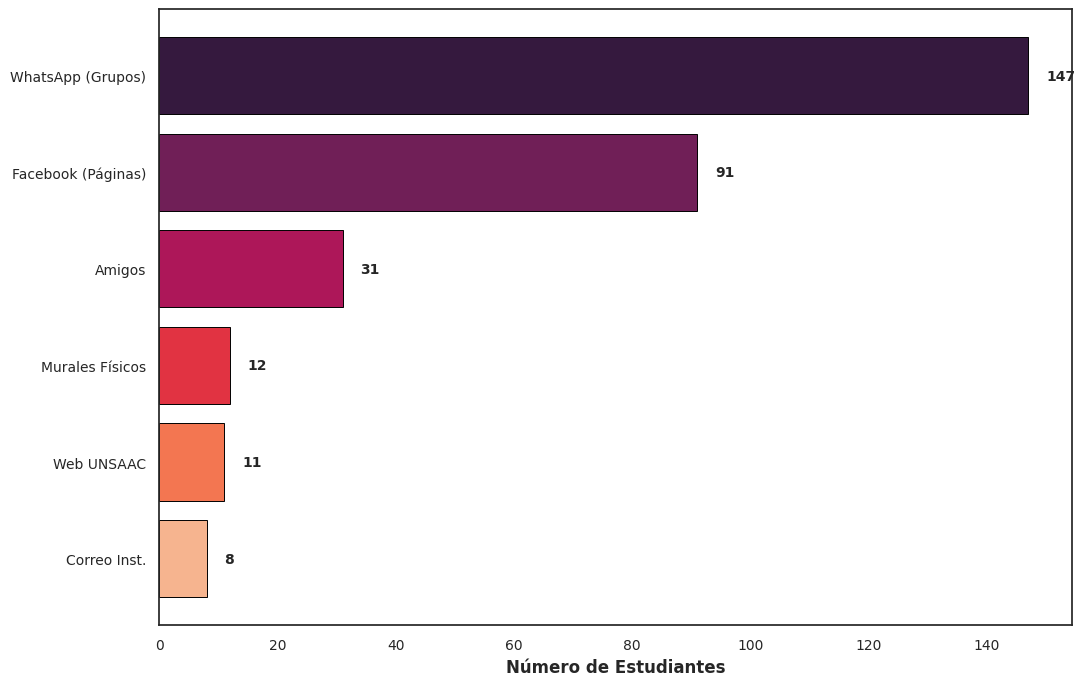
\includegraphics[width=0.88\linewidth,height=8cm,keepaspectratio]{imagenes/encuesta_03.png}\par
\captionof{figure}{Canales principales utilizados por las personas encuestadas}\label{fig:enc3}
\vspace{0.3cm}
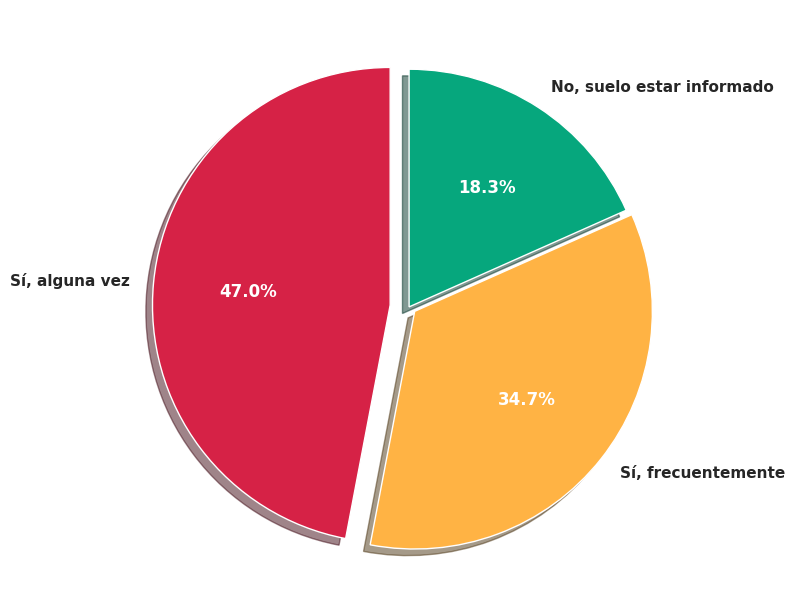
\includegraphics[width=0.88\linewidth,height=8cm,keepaspectratio]{imagenes/encuesta_04.png}\par
\captionof{figure}{Fechas importantes omitidas por falta de información oportuna}\label{fig:enc4}
\end{center}

\subsection{Alternativas para el servicio y la alimentación}
\textbf{A0. Mejora de canales existentes.} Ordenar fuentes, responsabilidades y una página central de avisos; difundir enlaces y QR mediante recursos disponibles. Es la comparación de menor equipamiento adicional.

\textbf{A1. Servicio interactivo con red eléctrica.} Añadir CMS, cliente público, tres terminales táctiles y respaldo dimensionado. Se evalúa si el acceso visible en espacios comunes aporta utilidad sobre A0.

\textbf{A2. Servicio interactivo con alimentación solar híbrida.} Integrar las funciones de A1 con generación FV, almacenamiento y gestión del circuito de cargas críticas. El conjunto de respaldo reemplaza los componentes equivalentes de A1; su costo se compara sobre la misma autonomía objetivo.

\cuadro{tab:alternativas}{Comparación preliminar de alternativas}{@{}P{3.0cm}Y Y Y@{}}{\textbf{Criterio}&\textbf{A0}&\textbf{A1}&\textbf{A2}}{
Información confiable & Depende de ordenar edición y fuentes & CMS y consulta trazable & Mismo beneficio informativo de A1\\*
Acceso presencial & Medios existentes y móvil & Tres puntos táctiles y QR & Igual cobertura física de A1\\
Complejidad & Menor integración & Cliente, red, soporte y energía & Añade FV, batería y estructura\\
Continuidad & Depende de medios existentes & Respaldo según carga & Respaldo central, FV y red de apoyo\\
Carga económica & Horas editoriales y canales & Equipos y servicio TI & A1 más inversión y operación solar\\
Decisión & Comprobar si resuelve la brecha & Demostrar valor de terminales & Justificar aporte y costo incremental\\
}
Se plantean dos decisiones: primero, si los terminales aportan valor frente a A0; después, si la generación aprovechada y las diferencias de desempeño justifican el incremento sobre A1.

Se formula A2 como alternativa integral del piloto y se conserva A1 como opción de ejecución por etapas. La decisión de inversión aplicará las reglas de comparación económica, capacidad operativa y aceptación técnica desarrolladas en el informe.

\subsection{Oferta y criterio de evaluación}
La oferta se compara por terminal completo, sistema soportado, orientación, cliente, energía, garantía y entrega en Cusco. El menor precio no determina cumplimiento. Las fichas oficiales respaldan características; las publicaciones comerciales respaldan sólo los importes y condiciones que explicitan.

Un tótem incluye pantalla, táctil, cómputo, carcasa y base. No se compara su precio con el de una pizarra horizontal o monitor suelto. Se solicitará una oferta homogénea para tres unidades, instalación y prueba, con impuestos, licencias y exclusiones explícitos.

\subsection{Comparación de terminales interactivos completos}
La unidad de comparación es el tótem vertical de piso con pantalla, superficie táctil, cómputo integrado, carcasa y base. Para la consulta interior se propone un mínimo de 55 pulgadas, resolución 4K, diez contactos táctiles y 400 cd/m\textsuperscript{2}; se prefieren 450 a 500 cd/m\textsuperscript{2} cuando la iluminación lo requiera. El ensayo en cada ubicación comprobará lectura, reflejos, altura y circulación.

El cuadro \ref{tab:fichas-totems} reúne cuatro ofertas publicadas en Perú y consultadas el 30 de octubre de 2026. Cada columna registra sólo lo que publica el vendedor, con su imagen referencial, precio, condición tributaria y los enlaces del producto y de la imagen. \emph{No publicado} indica un dato que la oferta deberá acreditar.

\begin{table}[p]\formatofichas
\caption{Tótems interactivos de 55 pulgadas analizados como opción}\label{tab:fichas-totems}
\begin{tabularx}{\linewidth}{@{}>{\raggedright\arraybackslash}p{2.15cm}YYYY@{}}
\toprule
\textbf{Característica} & \textbf{Prodimer TIPI7-55} & \textbf{First View FVD-D550M} & \textbf{Touch Data ADV5531, opción Pro} & \textbf{Visionsystems 55, Core i5}\\\midrule
\textbf{Imagen referencial} & \imgficha{imagenes/mercado_totem_prodimer.jpg}{3.0cm} & \imgficha{imagenes/mercado_totem_firstview.jpg}{3.0cm} & \imgficha{imagenes/mercado_totem_touchdata.jpg}{3.0cm} & \imgficha{imagenes/mercado_totem_visionsystems.jpg}{3.0cm}\\
\textbf{Proveedor} & Corporación Prodimer Perú S.A.C. & Perú Data Consult E.I.R.L., RUC 20486468913 & Touch Data Solutions & Visionsystems Perú, RUC 20511030332\\
\textbf{Procesador} & Core i7 de 13.\textsuperscript{a} generación; SKU no publicado & Core i7 de 13.\textsuperscript{a} generación; SKU no publicado & 13.\textsuperscript{a} generación; otras opciones: 8.\textsuperscript{a}, 6.\textsuperscript{a} y Android & Core i5; generación no publicada\\
\textbf{Memoria y SSD} & 16 GB; 256 GB & 16 GB DDR4; 256 o 512 GB & No publicados & No publicados\\
\textbf{Sistema} & Windows 11 Original; edición no publicada & Windows 11 Pro licenciado de fábrica & Windows con licencia; edición no publicada & Windows o Android; licencia no publicada\\
\textbf{Pantalla} & 3\,840 $\times$ 2\,160; 400 a 450 cd/m\textsuperscript{2} & LED 3\,840 $\times$ 2\,160; 450 cd/m\textsuperscript{2} & 4K vertical; brillo no publicado & 4K vertical; brillo no publicado\\
\textbf{Táctil} & Infrarrojo, 20 puntos & 20 puntos; la página indica infrarrojo y capacitivo & Infrarrojo, 10 puntos & Infrarrojo, 10 puntos\\
\textbf{Red, puertos y audio} & Wi-Fi 6, BT 5.4, RJ45, HDMI, VGA y USB 3.0 & Ethernet Gigabit, Wi-Fi 6, BT, HDMI, USB 3.0 y USB-C; parlantes de 8 W & No publicados & No publicados\\
\textbf{Energía y medidas} & 95 W sin condición de medición; medidas no publicadas & 100 a 240 V CA; 1\,900 $\times$ 850 $\times$ 100 mm; 85 kg brutos & No publicados & No publicados\\
\textbf{Garantía y alcance} & No indicada en el producto; política general de 36 meses & 3 años con el fabricante; producto a pedido & 1 año; incluye el software Touch Data Sign & 12 meses; entrega, instalación y software aparte\\
\textbf{Precio publicado} & S/~9\,499,99 por transferencia o S/~9\,974,99 con tarjeta; IGV no indicado & S/~10\,299,00; antes S/~11\,099,00; IGV no indicado & S/~7\,556,00 a S/~10\,794,00 + IGV según opción & S/~9\,999,00 con impuestos; 4 unidades disponibles\\
\textbf{Cota unitaria con IGV} & S/~11\,209,99 si fuera neto & S/~12\,152,82 si fuera neto & S/~12\,736,92 en el extremo superior & S/~9\,999,00 sin instalación ni software\\
\textbf{Enlace del producto} & \enlace{https://prodimerperu.com/producto/totem-interactivo-55-prodimer-peru/} & \enlace{https://www.perudataconsult.net/products/totem-interactivo-aio-electronics-55-touch-core-i7-13va-16gb-ddr4-ssd-256gb-w11pro-1-ano-fvd-d550m} & \enlace{https://touchdata.pe/producto/totem-vertical-touch-55/} & \enlace{https://visionsystemsperu.com/producto/totems-pantallas-publicitarias-leds-interactivos-touchs-screen-55-windows-android/}\\
\bottomrule
\end{tabularx}
\fuentefichas{Páginas de producto consultadas el 30 de octubre de 2026 \cite{prodimer,firstview,touchdata,visionsystems}. La cota con IGV aplica 18\% cuando la página no declara el tributo \cite{igv}. Fuente de las imágenes, de izquierda a derecha: \url{https://prodimerperu.com/wp-content/uploads/2026/06/TOTEM-PRODIMER-55-2.jpg}; \url{https://www.perudataconsult.net/cdn/shop/files/totem-1_9079a4dd-b94a-46e5-a063-dfc98ec8256e.jpg?v=1758993488}; \url{https://touchdata.pe/wp-content/uploads/2017/05/totem55webvj.jpg}; \url{https://visionsystemsperu.com/wp-content/uploads/2026/01/foto3.jpg}. Las imágenes son referenciales, se reproducen con fines académicos y su procedencia se registra en \texttt{procedencia\_imagenes.json}.}
\end{table}

\textbf{Opción elegida para valorizar ET-01: TIPI7-55}, porque publica la configuración Windows completa de menor precio con CPU admitida, brillo y táctil acreditados. Su política general de 36 meses de garantía rige sólo para bienes de fabricación propia, por lo que la oferta deberá declarar la garantía del tótem. Con la reserva tributaria y la reserva de licencia del presupuesto, la cota por terminal es S/~11\,559,99. First View documenta mejor licencia, garantía, medidas y masa, aunque su página alterna los códigos FVD-D550M y FVD-DS550M; con IGV incluido queda bajo esa cota y, si su precio fuera neto, la supera en S/~592,83 por unidad. Touch Data publica un rango con IGV aparte e incluye su propio CMS, no requerido en el escenario base. La oferta de Visionsystems no acredita brillo, memoria ni almacenamiento y excluye instalación y software. La contingencia cubre el peor caso de las alternativas comparadas; la selección se hará con ofertas homogéneas. La oferta final precisará procesador, edición y licencia del sistema, jornada admitida, potencia máxima del conjunto, base, anclajes y garantía.

La ruta GCS ADV-5542 de la versión anterior se retira de la comparación: su publicación en Sodimac figura sin existencias y sin precio \cite{gcstnt}. Hikvision DS-D6055UT-D/S se conserva como referencia documental de la ruta Android: Android 13, 4 GB/32 GB eMMC, 500 cd/m\textsuperscript{2}, 108 W típicos y 155 W máximos; no se encontró precio publicado en Perú \cite{hikvision}. La política de envío de Prodimer a provincias contempla agencia y flete en destino; se costearán transporte, descarga, instalación y atención en Cusco \cite{prodimer}.

\subsection{Matriz de cumplimiento y condición de suministro}
\textbf{C} indica acreditación documental en la ficha o publicación identificada; \textbf{P}, confirmación pendiente en la configuración ofertada o en su ensayo. La recepción comprobará el equipo entregado y el servicio integrado.

\cuadro{tab:mercado-cumplimiento}{Cumplimiento documental de los mínimos propuestos}{@{}Y P{1.95cm}P{1.95cm}P{1.95cm}P{1.95cm}@{}}{\textbf{Condición}&\textbf{Prodimer}&\textbf{First View}&\textbf{Touch Data}&\textbf{Vision\-systems}}{
55 pulgadas y estructura vertical de piso & C & C & C & C\\*
Pantalla 4K & C & C & C & C\\
Brillo de al menos 400 cd/m\textsuperscript{2} para interior & C & C: 450 & P & P\\
Diez contactos táctiles como mínimo & C: 20 & C: 20 & C: 10 & C: 10\\
CPU admitida por Windows 11; RAM y SSD declarados & C & C & P: RAM y SSD & P: generación, RAM y SSD\\
Sistema y licencia aptos para el cliente elegido & P & C: 11 Pro & P & P\\
Potencia máxima del terminal completo & P & P & P & P\\
Garantía del conjunto y atención en Cusco & P & P: 3 años & P: 1 año & P: 12 meses\\
Tratamiento tributario explícito & P & P & C: + IGV & C: incluido\\
Tres unidades, transporte e instalación en Cusco & P & P & P & P\\
}

La configuración Windows requerirá \textbf{Windows 11 Pro o una edición equivalente con licencia acreditada y funciones de bloqueo compatibles con el cliente}. Se incorpora una \textbf{reserva propia de S/ 350 por terminal, S/ 1\,050 en total}, para cerrar la edición y el derecho de uso cuando no estén incluidos en la oferta. Esta provisión se conciliará con el suministro para evitar duplicidades.

La mantenibilidad se evaluará mediante actualizaciones documentadas para un \textbf{horizonte objetivo de cinco años}, disponibilidad de controladores y repuestos, acceso técnico y una ruta de renovación del cliente. Windows 10 llegó al fin de soporte el 14 de octubre de 2025, sin asistencia técnica ni actualizaciones de seguridad posteriores \cite{win10fin}; no se aceptarán terminales con ese sistema. La lista de procesadores Intel admitidos por Windows 11 comienza en la 8.\textsuperscript{a} generación Core \cite{win11cpu}: la opción de 6.\textsuperscript{a} generación queda excluida y la de 8.\textsuperscript{a} requerirá soporte acreditado para el horizonte. Se exigirán exportación de contenidos y datos, separación entre administración y consulta pública y gestión de destinos por terminal. El horizonte constituye un criterio de planificación; el plazo contractual de garantía se establecerá por componente. La capacidad de CPU, RAM y almacenamiento se aceptará por el rendimiento del servicio, sin exigir la gama máxima.

\subsection{Fuentes de precio y catálogos electrónicos}
Los importes de este estudio son precios publicados por vendedores identificados. Sirven para la indagación de mercado de la formulación; no constituyen ofertas ni sustituyen las cotizaciones que solicite la entidad. Antes de convocar, el órgano encargado de las contrataciones verificará si los bienes figuran en los Catálogos Electrónicos de Acuerdos Marco, cuyo uso es obligatorio para los bienes catalogados, salvo las excepciones previstas \cite{contrataciones}.

El Buscador de Fichas de Producto de PERÚ COMPRAS informaba, con datos actualizados al 29 de octubre de 2026, 14 acuerdos marco de bienes vigentes y 26 catálogos. Son pertinentes EXT-CE-2024-2 Equipos multimedia y accesorios, EXT-CE-2022-5 Computadoras de escritorio, computadoras portátiles y escáneres, EXT-CE-2024-14 Luminarias, materiales eléctricos y cables eléctricos y EXT-CE-2024-1 Baterías, pilas y accesorios \cite{perucompras}. La verificación se hará por ficha-producto: el nombre de un catálogo no acredita que incluya un tótem de 55 pulgadas, un módulo FV, un inversor híbrido o el material eléctrico especificado.

La indagación comparará al menos dos ofertas homogéneas por componente. Cada una identificará proveedor y RUC, modelo exacto, moneda, impuestos, vigencia, plazo y lugar de entrega, garantía y exclusiones, con la fecha de consulta. Cuando la página comercial y la ficha del fabricante difieran, prevalecerá la ficha y la oferta deberá aclarar la diferencia.

\subsection{Alternativas de gestión de contenidos y costo del software}
Las tres rutas siguientes se evaluarán con las mismas funciones: permisos por grupo, preparación y revisión de avisos, programación y vencimiento, destinos, interacción táctil, consulta local y supervisión \cite{xibousers,xibotouch,xibodisplays}. La aprobación editorial deberá demostrarse con las cuentas y permisos configurados.

\cuadro{tab:mercado-cms}{Comparación de modalidades de CMS y reproductor}{@{}P{3.1cm}Y P{4.0cm}@{}}{\textbf{Modalidad}&\textbf{Operación y responsabilidad}&\textbf{Licencia o plan publicado}}{
CMS autoalojado y reproductor Windows & Administración del servidor, seguridad, copias, actualización del CMS y clientes a cargo del operador. Permite separar la plataforma de contenidos del terminal. & Núcleo y reproductor Windows abiertos bajo AGPLv3 o posterior, sin cargo por esas licencias \cite{xibolic}.\\*
CMS autoalojado y reproductor Android & Conserva las obligaciones del servidor; requiere instalación y prueba del reproductor en el SoC concreto. & USD 28 por reproductor perpetuo; tres: USD 84. Revisiones menores de la versión incluidas; actualización mayor según condiciones del fabricante \cite{xibolic}.\\
Xibo Cloud, plan Professional & Alojamiento del CMS, reproductor y soporte según el plan; el operador local conserva contenidos, equipos, conectividad y atención presencial. & USD 4,90 por pantalla-mes; tres: USD 14,70/mes y USD 176,40/año equivalentes \cite{xibolic}.\\
}

La base de software del presupuesto comprende \textbf{S/ 6\,000 para configuración y adaptación del CMS}, \textbf{S/ 3\,000 para interfaz y contenidos} y \textbf{S/ 720/año para alojamiento autoalojado}. Son estimaciones propias de planificación. La ausencia de cargo de licencia del software abierto mantiene las necesidades de configuración, operación y soporte. Al elegir un plan alojado se reemplazará la partida equivalente de alojamiento y se conciliará la licencia del reproductor. Los importes en USD se conservan en su moneda de publicación; facturación, conversión e impuestos se cerrarán al contratar.

\subsection{Prueba del cliente y criterio de selección tecnológica}
Xibo descarga medios, diseños y metadatos a una biblioteca local para reproducción sin conexión \cite{xibostorage}. El ensayo comprobará consulta, vencimiento, desconexión, reinicio sin red y actualización íntegra al reconectar. Una página externa integrada requerirá definir qué información se conserva localmente y cómo se valida su vigencia.

La ruta web o PWA deberá resolver ese mismo comportamiento. Las experiencias de kiosco de Edge utilizan InPrivate \cite{edge}; la continuidad tras reinicio exige probar la persistencia de la configuración elegida y, cuando corresponda, emplear un reproductor con biblioteca persistente o un paquete local controlado \cite{pwa,xibostorage}.

La pantalla 4K se distingue de la resolución con que se dibuja la interfaz. La documentación de Xibo para Android describe interfaz, imágenes y contenido web en 1080p escalados al panel 4K, con video nativo 4K \cite{xiboresolution}. La decisión valorará legibilidad y respuesta en el tótem real, sin prometer una interfaz nativa 4K por la resolución de la pantalla.


